Odată ce o cerere de începere a unei execuții a unui workflow este primită de către crawler, funcția Lambda corespunzatoare începerii execuției (i.e. \textit{"Pornire workflow"}) este invocată. Aceasta creează și salvează metadatele necesare în baza de date (e.g. timpul la care a inceput workflow-ul, cu scopul de a putea contoriza cât a durat execuția), apoi invocă funcția Lambda responsabilă pentru inițializarea mecanismului de distribuție și sincronizare a execuției în paralel a funcțiilor ce parcurg paginile web. \textit{"Figura 7"} descrie modul în care funcția de inițializare a unui workflow este utilizată, precum și rolul pe care aceasta îl îndeplinește în procesul recursiv de crawling.

\begin{figure}[ht]
\begin{center}
	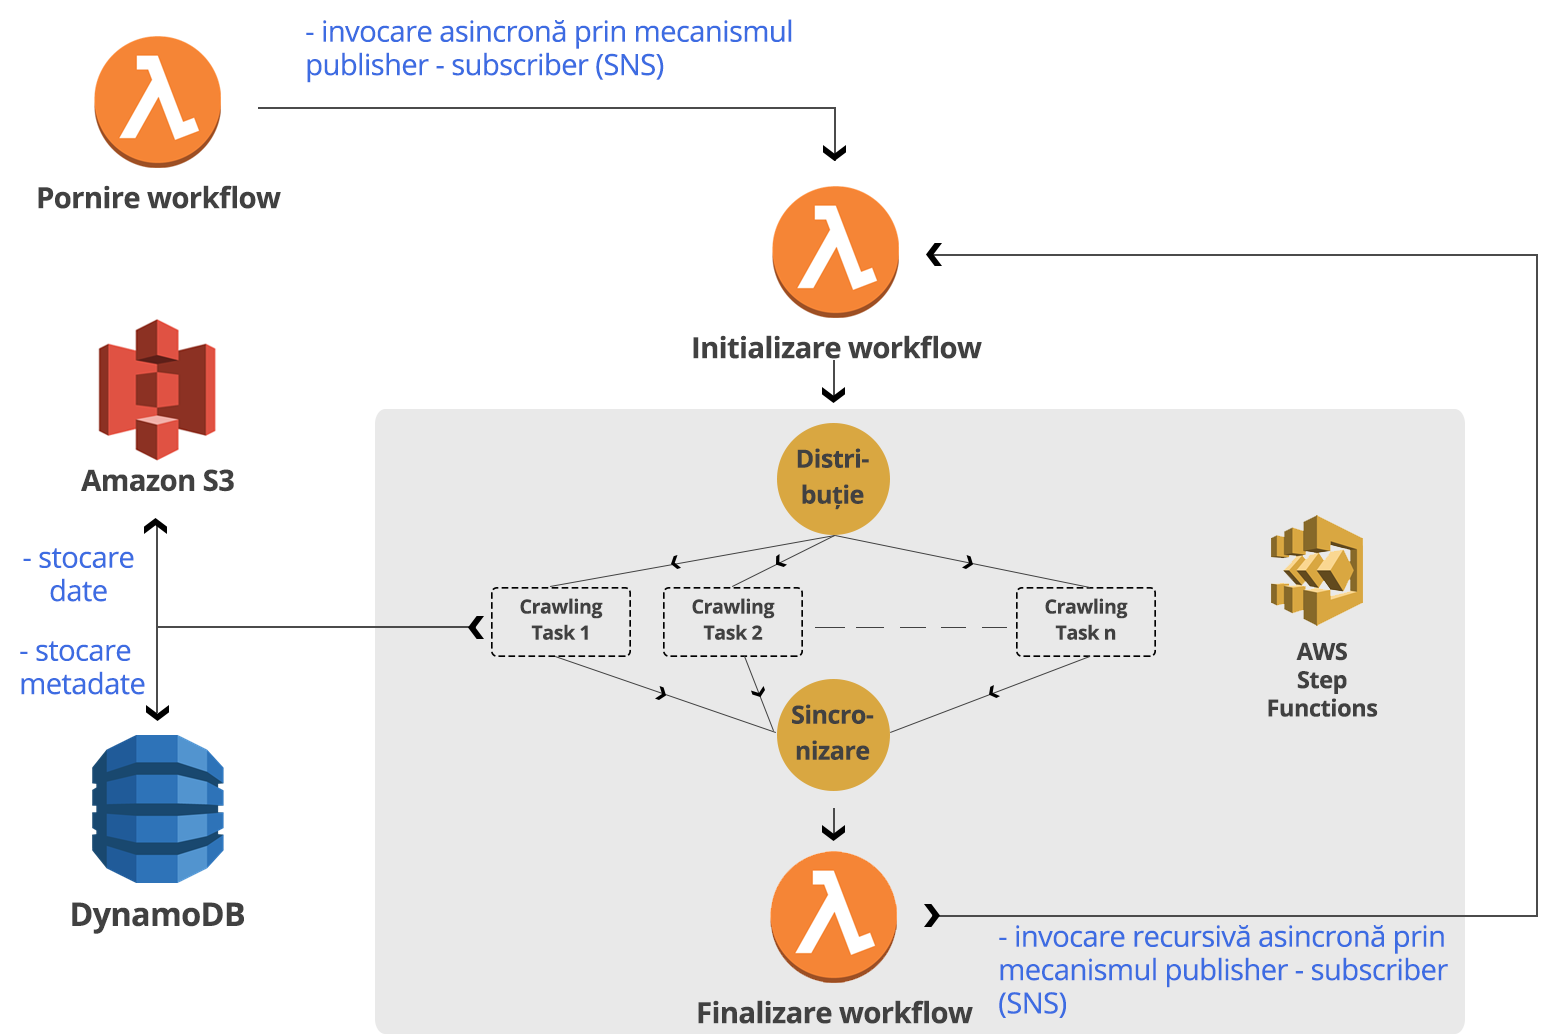
\includegraphics[keepaspectratio, width=1.0\textwidth]{proces-crawling-high-level.png}
	\caption{Arhitectura unui workflow \cite{diagram-icons-sources, aws-icons-source}}\par\medskip 

\end{center}
\end{figure}

\noindent
Responsabilitățile funcției de inițializare a workflow-ului sunt următoarele:

\begin{itemize}
	\item{Verificarea nivelului de adâncime la care s-a ajuns în urma procesului de crawling și finalizarea workflow-ului, în caz că nivelul de adâncime maxim a fost depășit;}
	\item{Interogarea bazei de date în vederea extragerii task-urilor pentru parcurgerea paginilor web, task-uri ce sunt executate în cadrul automatului orchestrat de către "AWS Step Functions";}
	\item{Crearea și pornirea automatului finit construit în cadrul "AWS Step Functions", pe baza task-urilor extrase din baza de date. Acest automat este definit prin două stagii secvențiale. Primul stagiu are ca scop orchestrarea distribuită a sarcinilor de crawling executate în paralel, iar cel de-al doilea are ca scop agregarea, interpretarea și salvarea datelor provenite din execuția task-urilor concurente.}
\end{itemize}
